\begin{appendices}
\chapter{Manual de usuario}\label{anexo:manual_de_usuario}

El presente manual de usuario tiene como objetivo proporcionar una guía detallada y visual para la utilización de la plataforma \textit{Quizzie}. A diferencia de un catálogo estático de pantallas, este documento estructura la guía siguiendo la experiencia de usuario cronológica real: desde el punto de entrada a la aplicación web y el acceso diferenciado por roles, hasta la navegación por el panel principal, la preparación de contenidos y el desarrollo completo de una sesión interactiva en tiempo real.

\section*{Punto de entrada a la aplicación y roles de usuario}

Al navegar a la dirección raíz del sitio web (\texttt{/}), la plataforma ofrece una interfaz unificada adaptada a los dos perfiles principales:

\begin{itemize}
    \item[\tiny$\blacksquare$] \textbf{Alumno:} Accede directamente desde la pantalla de bienvenida introduciendo el código PIN proyectado en el aula, sin necesidad de contraseñas ni registros previos.
    \item[\tiny$\blacksquare$] \textbf{Profesor:} Dispone de accesos dedicados para iniciar sesión (\texttt{/login}) o registrarse (\texttt{/register}). Tras autenticarse, accede a un panel de control privado con una barra de navegación lateral (\textit{sidebar}) para gestionar sus cuestionarios y salas.
\end{itemize}

\section*{Registro, autenticación y gestión del perfil docente}

El ciclo de vida del usuario docente comienza desde la pantalla principal de la plataforma, guiando al profesor a través de un proceso de registro con correo electrónico, la administración de su cuenta y los mecanismos de recuperación de acceso.

\subsection*{1. Acceso inicial a la plataforma}

Al acceder a la aplicación web, el profesor visualiza la pantalla de inicio, la cual permite iniciar sesión o registrarse, o bien saltar a la zona de estudiantes.

\begin{figure}[H]
  \centering
  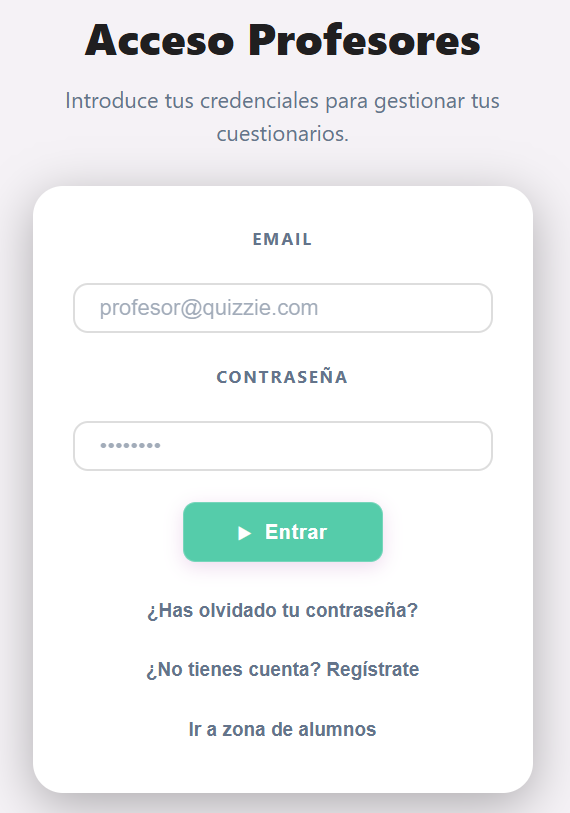
\includegraphics[width=0.42\textwidth]{screenshots/inicio.png}
  \caption{Punto de entrada a la plataforma.}
  \label{fig:manual_inicio}
\end{figure}

\subsection*{2. Formulario de registro docente}

Al pulsar sobre la opción de registro, el sistema presenta un formulario donde el profesor debe ingresar su nombre, dirección de correo electrónico y una contraseña.

\begin{figure}[H]
  \centering
  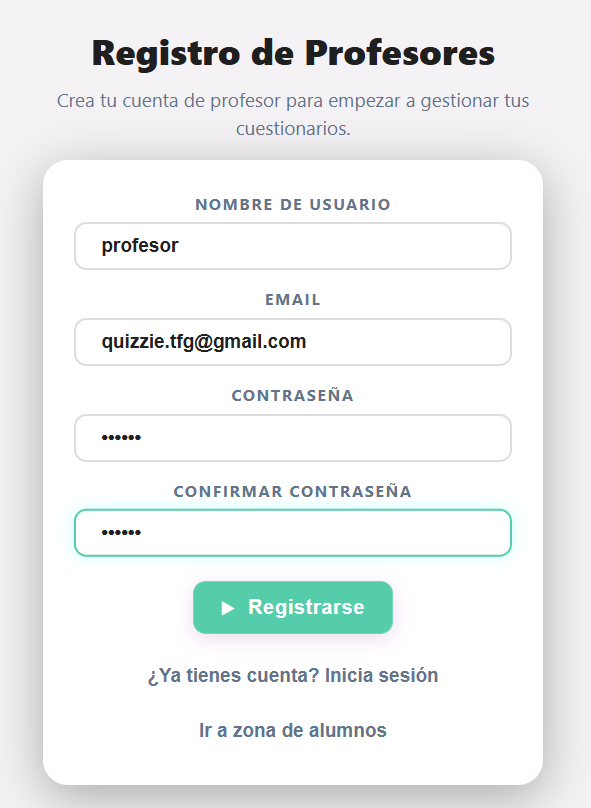
\includegraphics[width=0.44\textwidth]{screenshots/registro.png}
  \caption{Formulario de registro para el perfil docente.}
  \label{fig:manual_registro}
\end{figure}

\subsection*{3. Notificación de verificación de cuenta}

Una vez completado y enviado el formulario, la plataforma envía un correo electrónico a la dirección facilitada con un código numérico temporal de un solo uso para verificar la cuenta.

\begin{figure}[H]
  \centering
  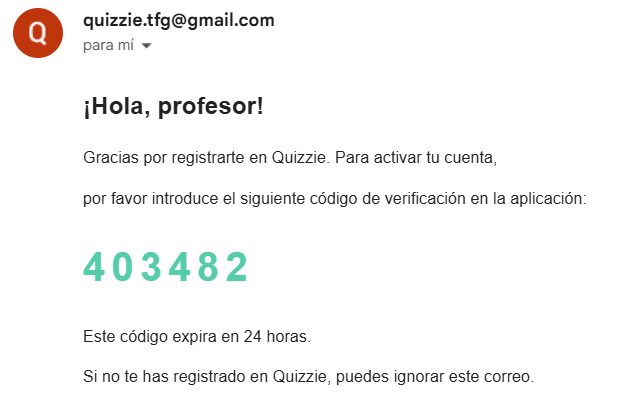
\includegraphics[width=0.6\textwidth]{screenshots/correo_verificar_cuenta.png}
  \caption{Correo electrónico con el código de verificación de cuenta.}
  \label{fig:manual_correo_verificar}
\end{figure}

\subsection*{4. Confirmación del código y activación}

El profesor es redirigido a una vista específica donde debe introducir el código recibido en el correo. Al pulsar sobre el botón de confirmación, la cuenta queda validada en la base de datos y habilitada para su uso.

\begin{figure}[H]
  \centering
  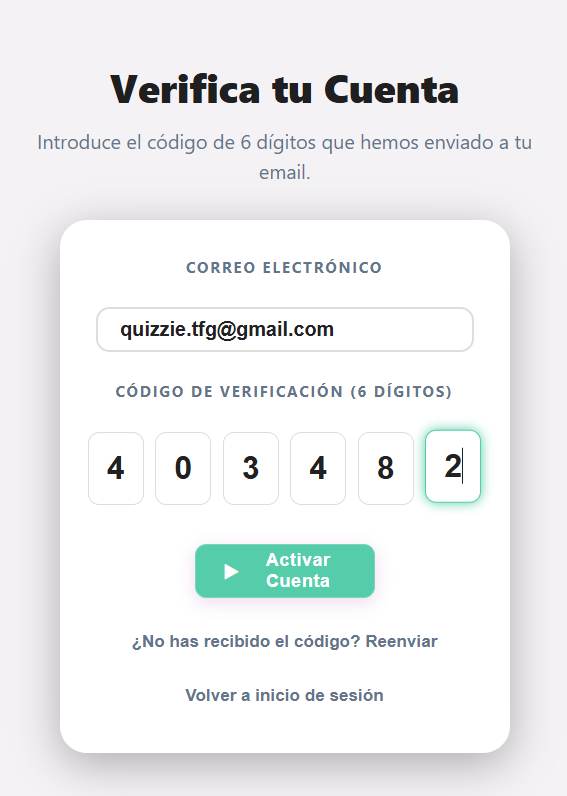
\includegraphics[width=0.42\textwidth]{screenshots/verificar_cuenta.png}
  \caption{Pantalla de introducción del código de verificación de cuenta.}
  \label{fig:manual_verificar_cuenta}
\end{figure}

\subsection*{5. Panel y opciones del perfil}

Tras iniciar sesión, el docente puede acceder a la sección de su perfil personal. Desde esta vista se muestran los datos del usuario y se facilitan las acciones de actualización de datos, cambio de contraseña o borrado de la cuenta.

\begin{figure}[H]
  \centering
  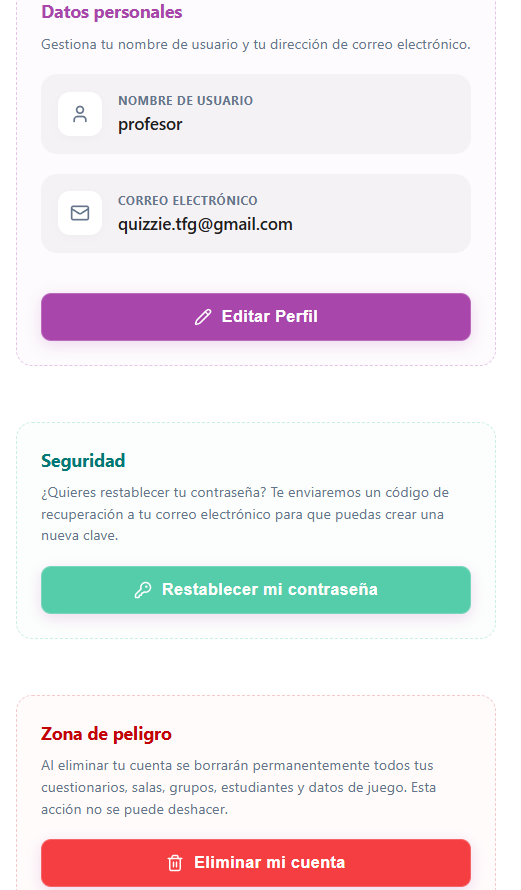
\includegraphics[width=0.6\textwidth]{screenshots/mi_perfil.png}
  \caption{Vista de gestión del perfil docente.}
  \label{fig:manual_mi_perfil}
\end{figure}

\subsection*{6. Solicitud y correo de restablecimiento de contraseña}

Si el profesor solicita una modificación o recuperación de contraseña, el sistema envía un nuevo correo electrónico que contiene el código de autorización requerido para efectuar dicho cambio.

\begin{figure}[H]
  \centering
  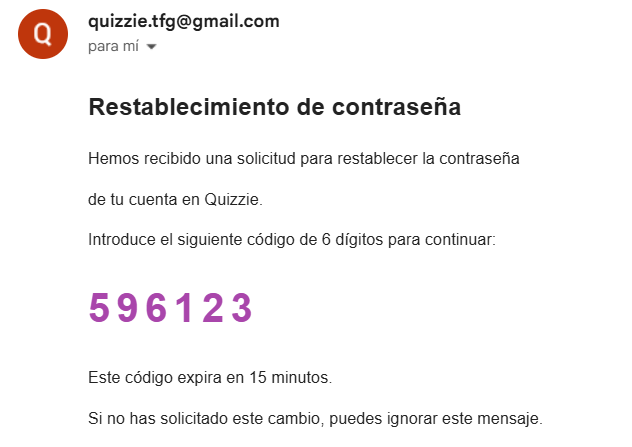
\includegraphics[width=0.62\textwidth]{screenshots/correo_cambiar_contra.png}
  \caption{Correo electrónico para el restablecimiento de contraseña.}
  \label{fig:manual_correo_cambiar_contra}
\end{figure}

\subsection*{7. Introducción de nueva contraseña}

En la interfaz, el usuario introduce el código de un solo uso recibido por correo junto con su nueva clave de acceso, efectuándose así la actualización de la contraseña.

\begin{figure}[H]
  \centering
  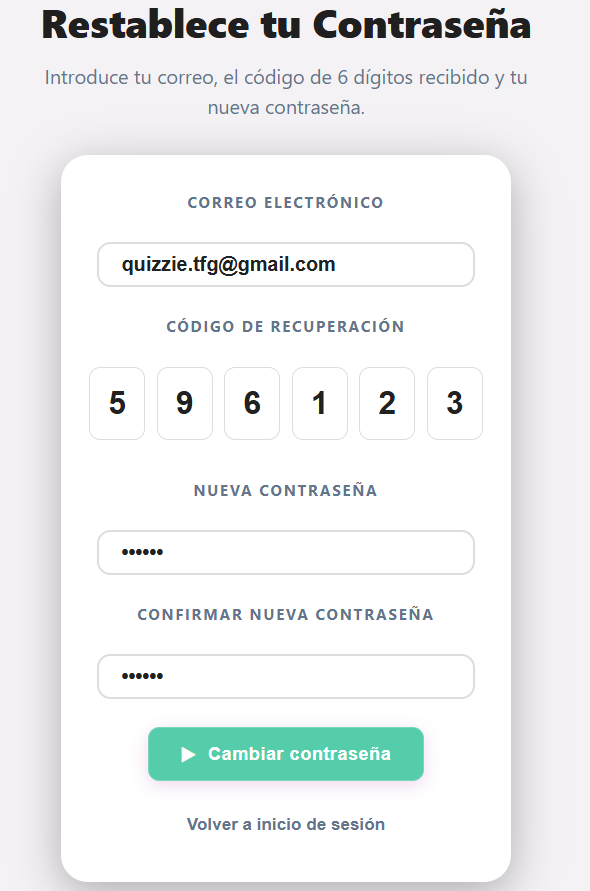
\includegraphics[width=0.45\textwidth]{screenshots/restablecer_contra.png}
  \caption{Formulario para establecer la nueva contraseña.}
  \label{fig:manual_restablecer_contra}
\end{figure}

\subsection*{8. Eliminación definitiva de la cuenta}

Finalmente, la plataforma contempla el derecho al borrado de datos. El docente puede solicitar la supresión completa de su perfil y datos asociados mediante un diálogo de confirmación que advierte sobre la irreversibilidad de la acción.

\begin{figure}[H]
  \centering
  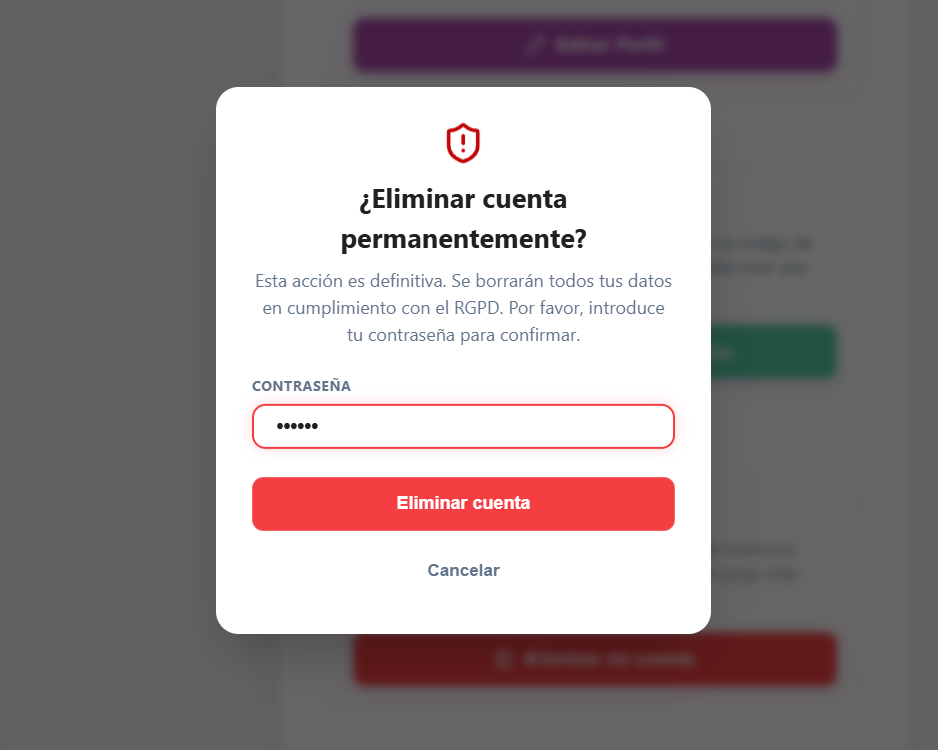
\includegraphics[width=0.85\textwidth]{screenshots/eliminar_cuenta.png}
  \caption{Confirmación de eliminación de la cuenta de usuario.}
  \label{fig:manual_eliminar_cuenta}
\end{figure}

\section*{Gestión del catálogo de cuestionarios e historial docente}\label{sec:manual_gestion_cuestionarios}

Una vez autenticado en la plataforma, el docente dispone de un entorno centralizado para la administración de sus contenidos académicos. Desde este espacio es posible consultar el catálogo de pruebas creadas, editar sus preguntas y parámetros, examinar las métricas de sesiones anteriores, exportar los resultados y crear nuevos cuestionarios.

\subsection*{1. Inicio de sesión del profesor}

El docente introduce su correo electrónico y contraseña en el formulario de acceso para ingresar a su panel privado de control.

\begin{figure}[H]
  \centering
  \makebox[\textwidth][c]{%
    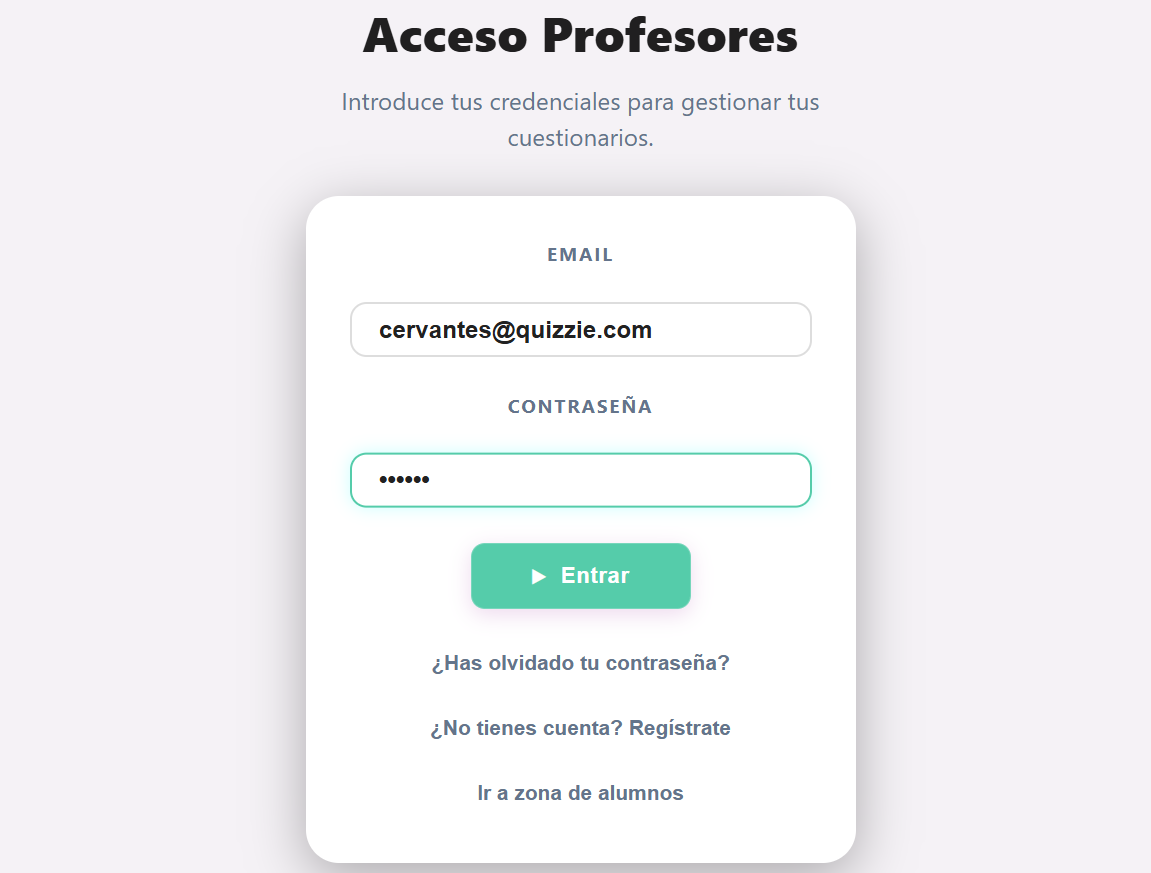
\includegraphics[width=0.8\textwidth]{screenshots/iniciar_sesion.png}%
  }
  \caption{Formulario de inicio de sesión.}
  \label{fig:manual_iniciar_sesion}
\end{figure}

\subsection*{2. Catálogo de cuestionarios disponibles}

Al acceder a la sección de cuestionarios, el profesor visualiza la lista con todas sus pruebas creadas. Cada entrada dispone de tres acciones rápidas: el icono del lápiz para modificar el cuestionario, el ojo para consultar el historial de salas asociadas y la papelera para su eliminación.

\begin{figure}[H]
  \centering
  \makebox[\textwidth][c]{%
    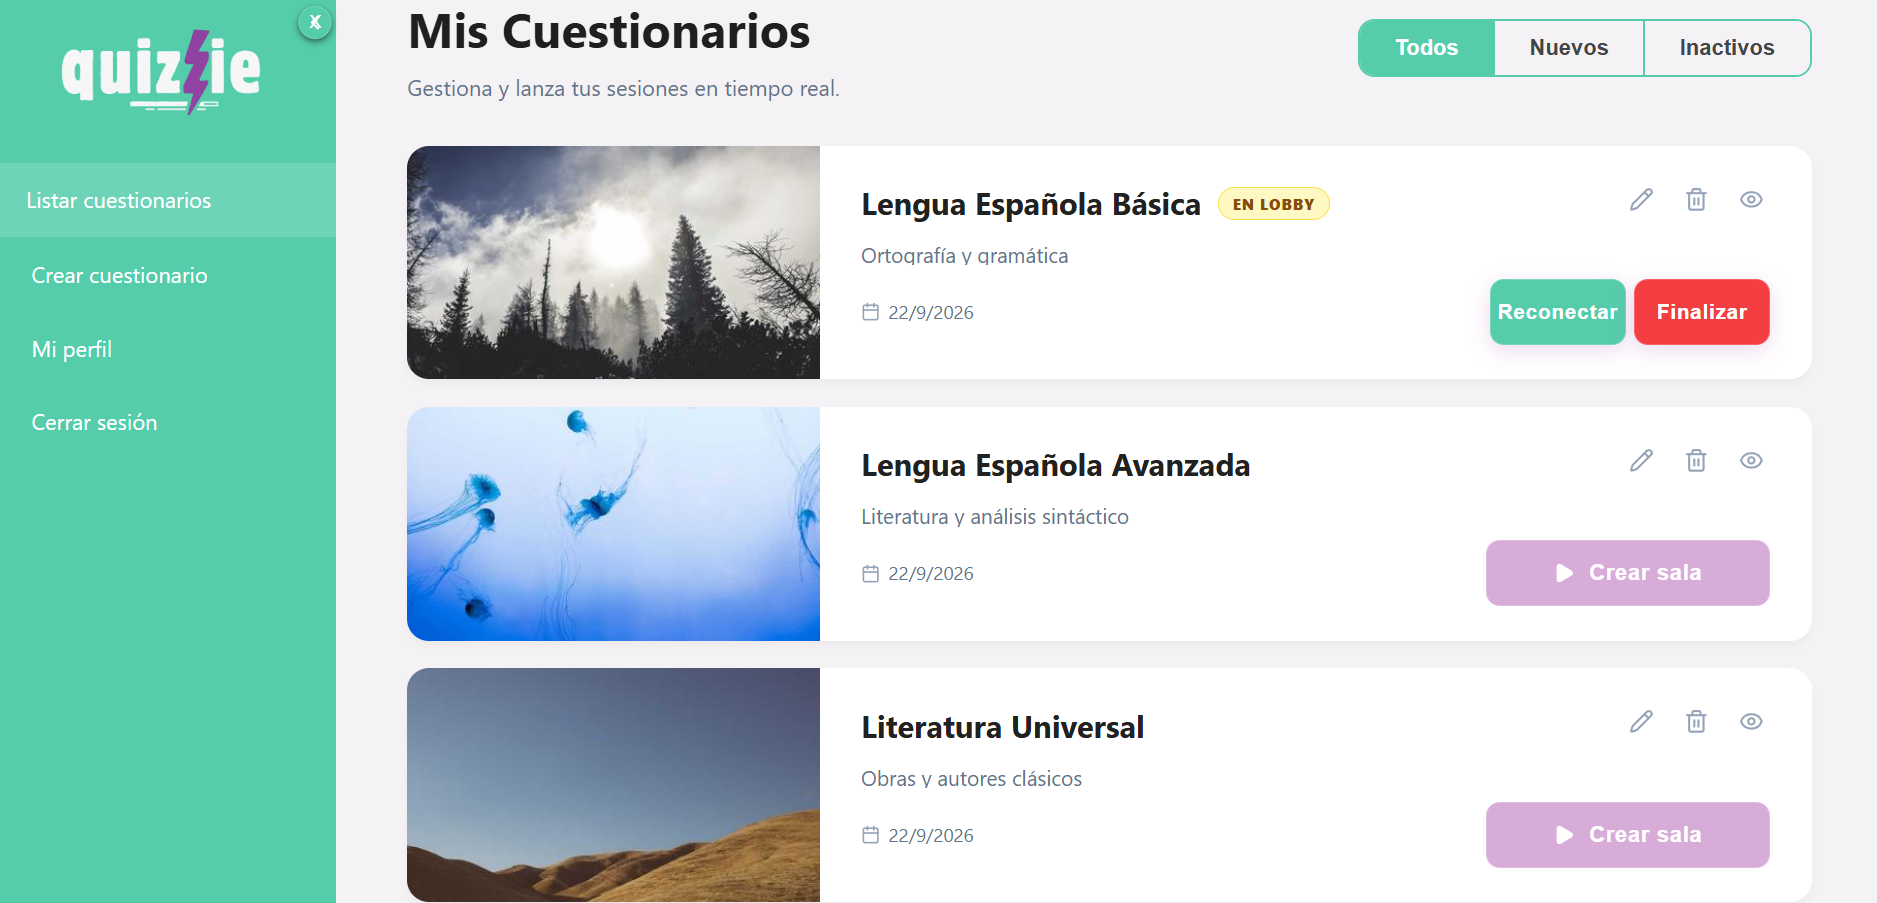
\includegraphics[width=1.1\textwidth]{screenshots/mis_cuestionarios.png}%
  }
  \caption{Listado general de cuestionarios del profesor.}
  \label{fig:manual_mis_cuestionarios}
\end{figure}

\subsection*{3. Edición de cuestionario}

Pulsando sobre el botón de edición, se abre el formulario donde es posible cambiar el título, modificar su descripción o ajustar el contenido, opciones y puntajes de las preguntas existentes.

\begin{figure}[H]
  \centering
  \makebox[\textwidth][c]{%
    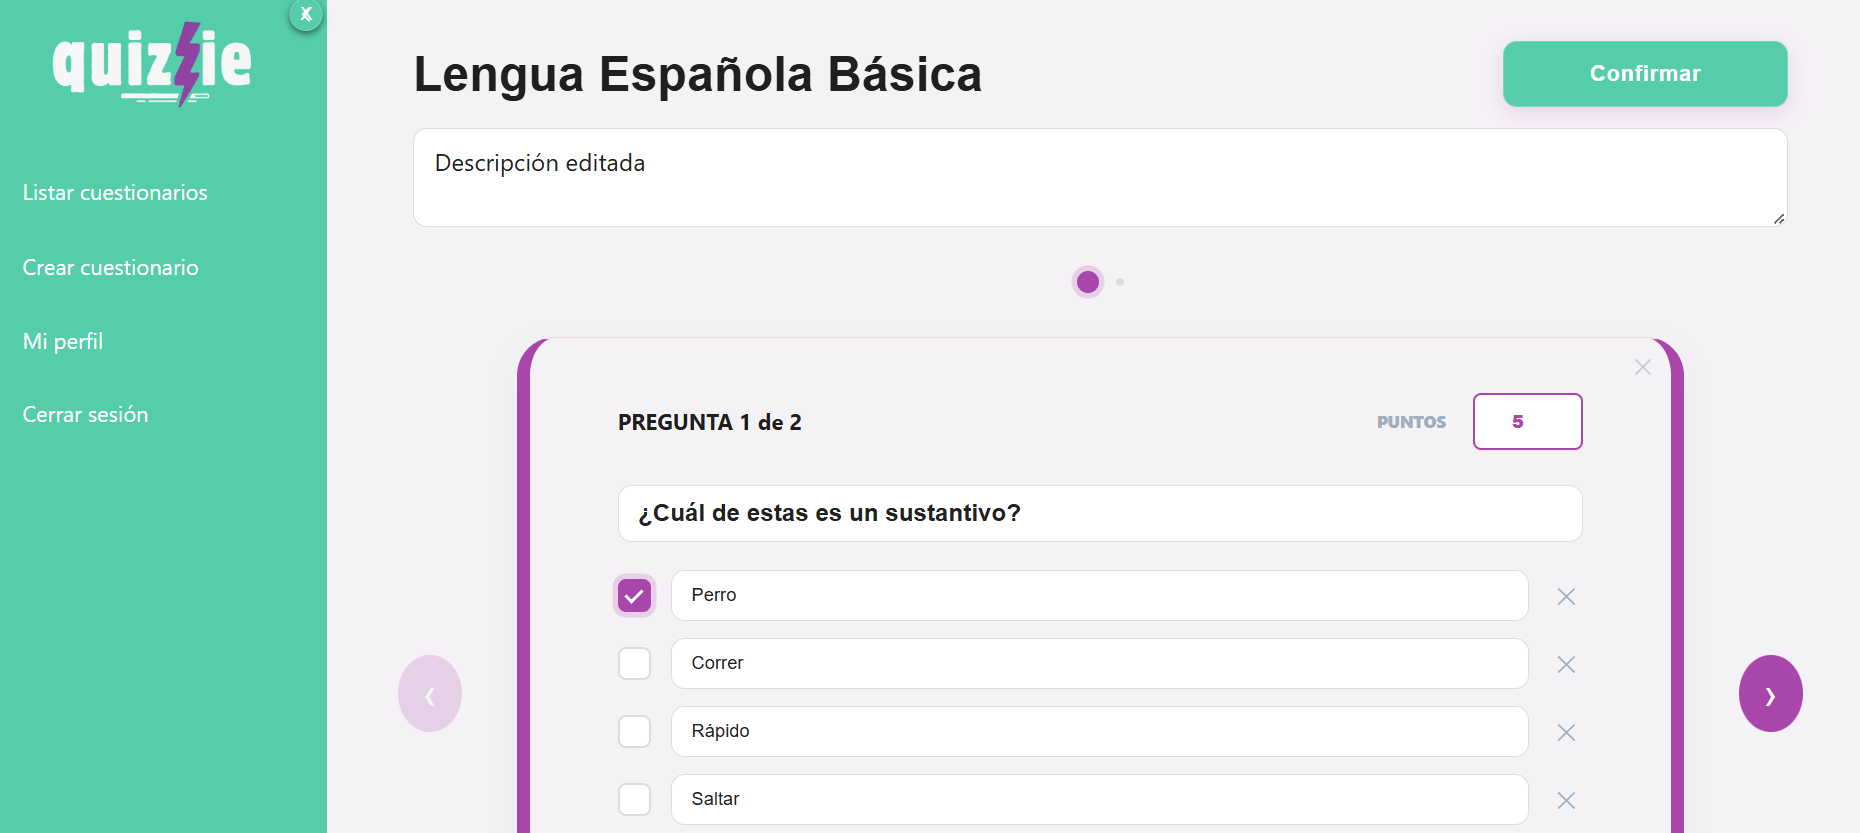
\includegraphics[width=1.1\textwidth]{screenshots/editar_cuestionario.png}%
  }
  \caption{Vista de edición de un cuestionario.}
  \label{fig:manual_editar_cuestionario}
\end{figure}

\subsection*{4. Historial de salas jugadas}

Al seleccionar la opción del ojo, el sistema presenta el registro histórico de las salas que se han disputado con dicho cuestionario. Al hacer clic sobre una sala concreta del listado, se accede al desglose pormenorizado de sus resultados.

\begin{figure}[H]
  \centering
  \makebox[\textwidth][c]{%
    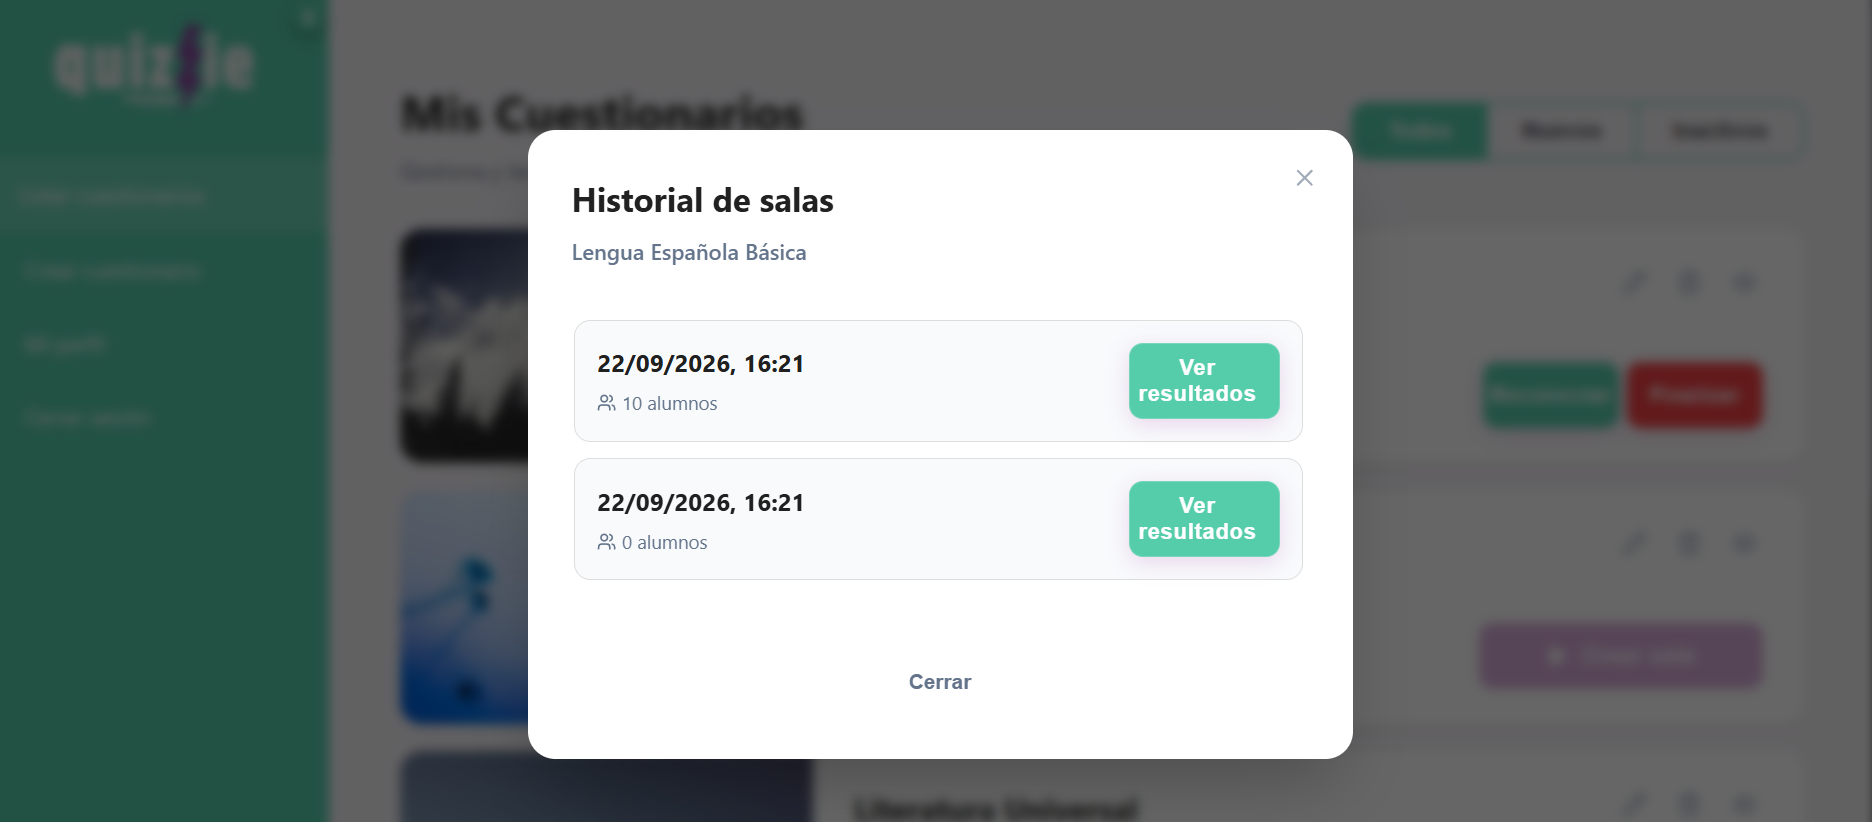
\includegraphics[width=1.1\textwidth]{screenshots/historial_salas.png}%
  }
  \caption{Historial de salas de un cuestionario.}
  \label{fig:manual_historial_salas}
\end{figure}

\subsection*{5. Detalle de resultados históricos y exportación}

En esta vista se muestran las puntuaciones registradas durante la sala seleccionada. Mediante el botón de descarga, el profesor puede exportar todo el conjunto de resultados a un archivo en formato CSV para su posterior tratamiento analítico o calificación externa.

\begin{figure}[H]
  \centering
  \makebox[\textwidth][c]{%
    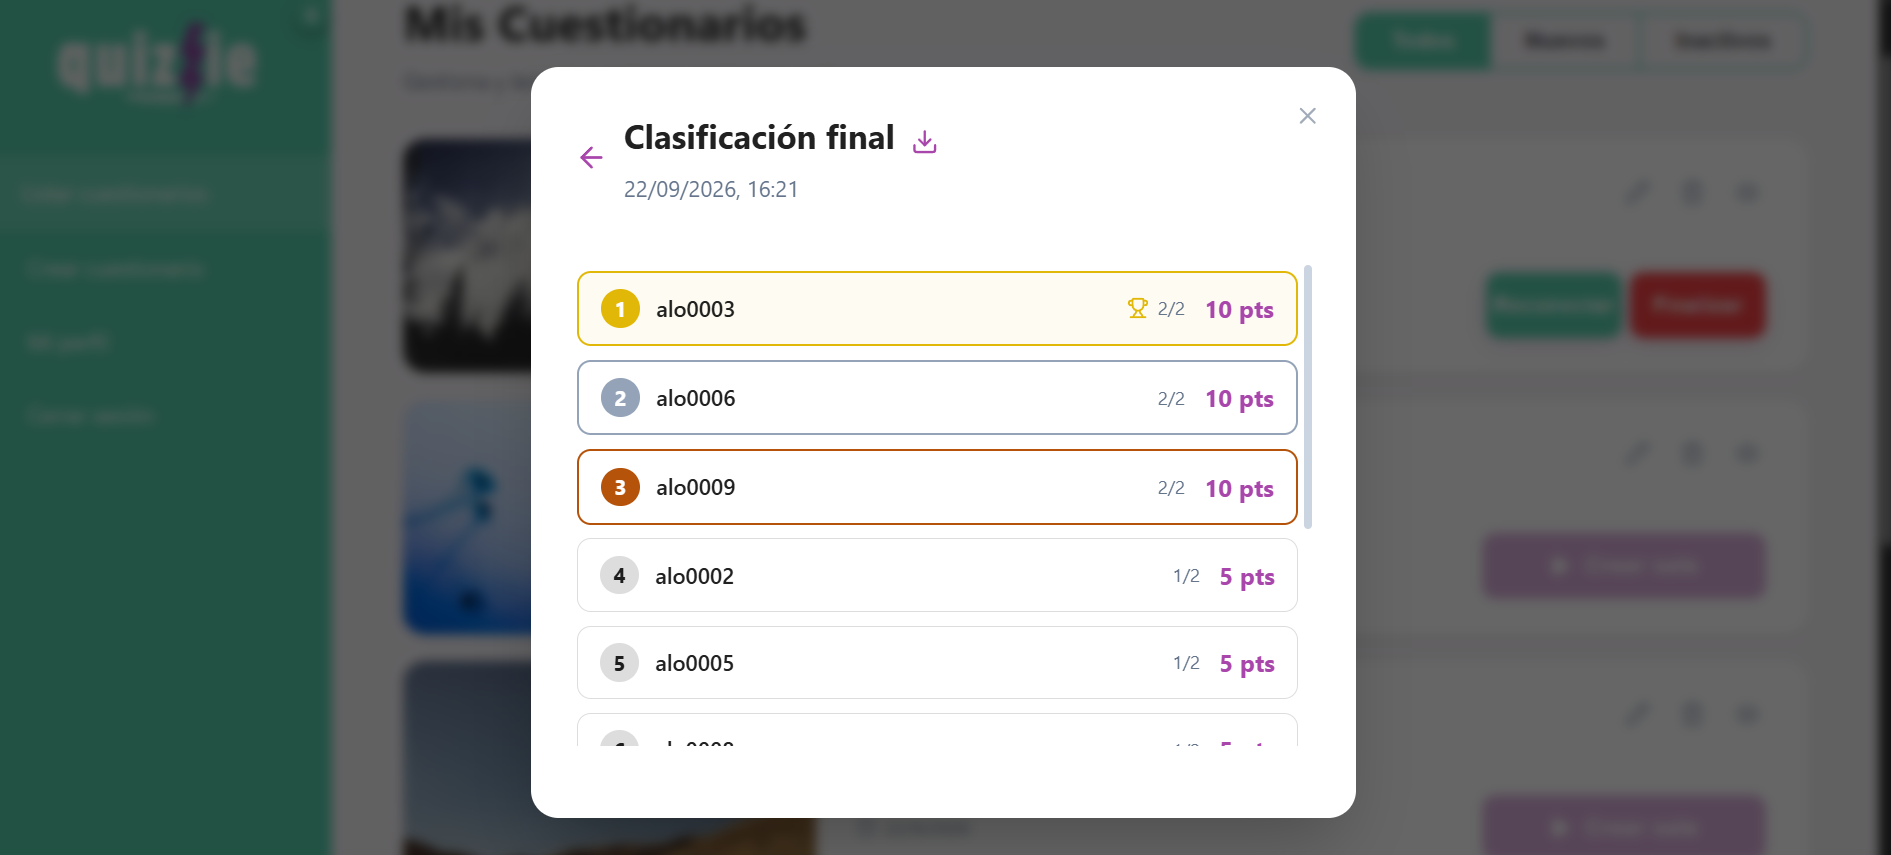
\includegraphics[width=1.1\textwidth]{screenshots/resultado_historico.png}%
  }
  \caption{Métricas detalladas de la sala y opción de exportación a CSV.}
  \label{fig:manual_resultado_historico}
\end{figure}

\subsection*{6. Eliminación de un cuestionario}

Al pulsar sobre el icono de la papelera, la plataforma solicita una confirmación previa para evitar pérdidas accidentales de datos antes de suprimir definitivamente el cuestionario.

\begin{figure}[H]
  \centering
  \makebox[\textwidth][c]{%
    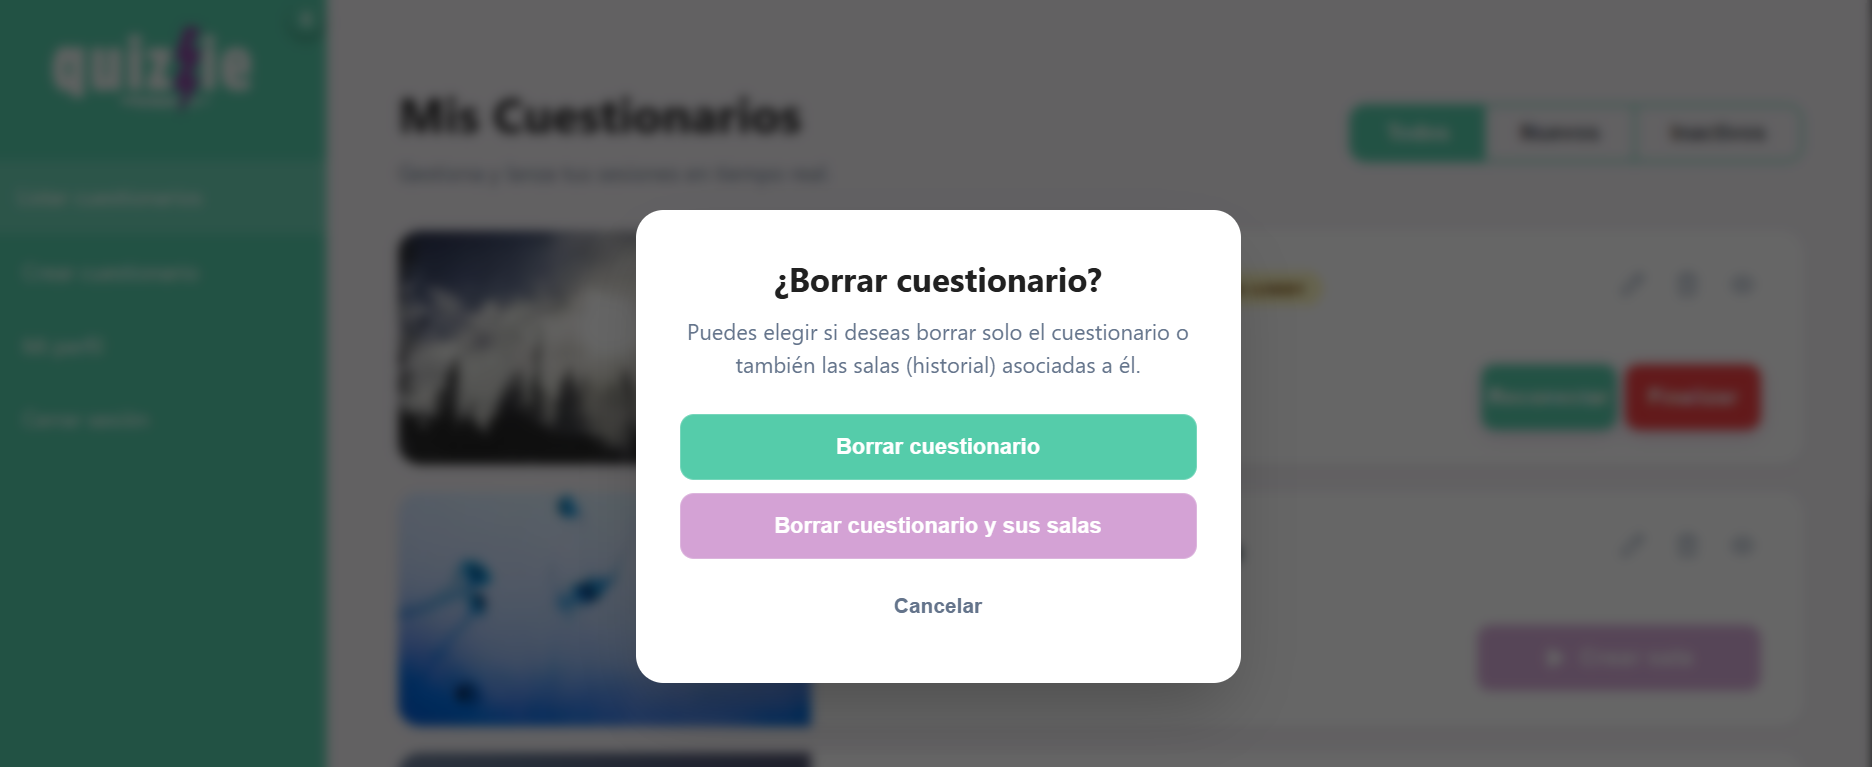
\includegraphics[width=1.1\textwidth]{screenshots/borrar_cuestionario.png}%
  }
  \caption{Diálogo de confirmación para eliminar un cuestionario.}
  \label{fig:manual_borrar_cuestionario}
\end{figure}

\subsection*{7. Creación de un nuevo cuestionario}

A través del botón de creación, el profesor accede a la interfaz de diseño de nuevos cuestionarios, donde define el título, las preguntas, las opciones de respuesta marcando la correcta y la puntuación máxima permitida.

\begin{figure}[H]
  \centering
  \makebox[\textwidth][c]{%
    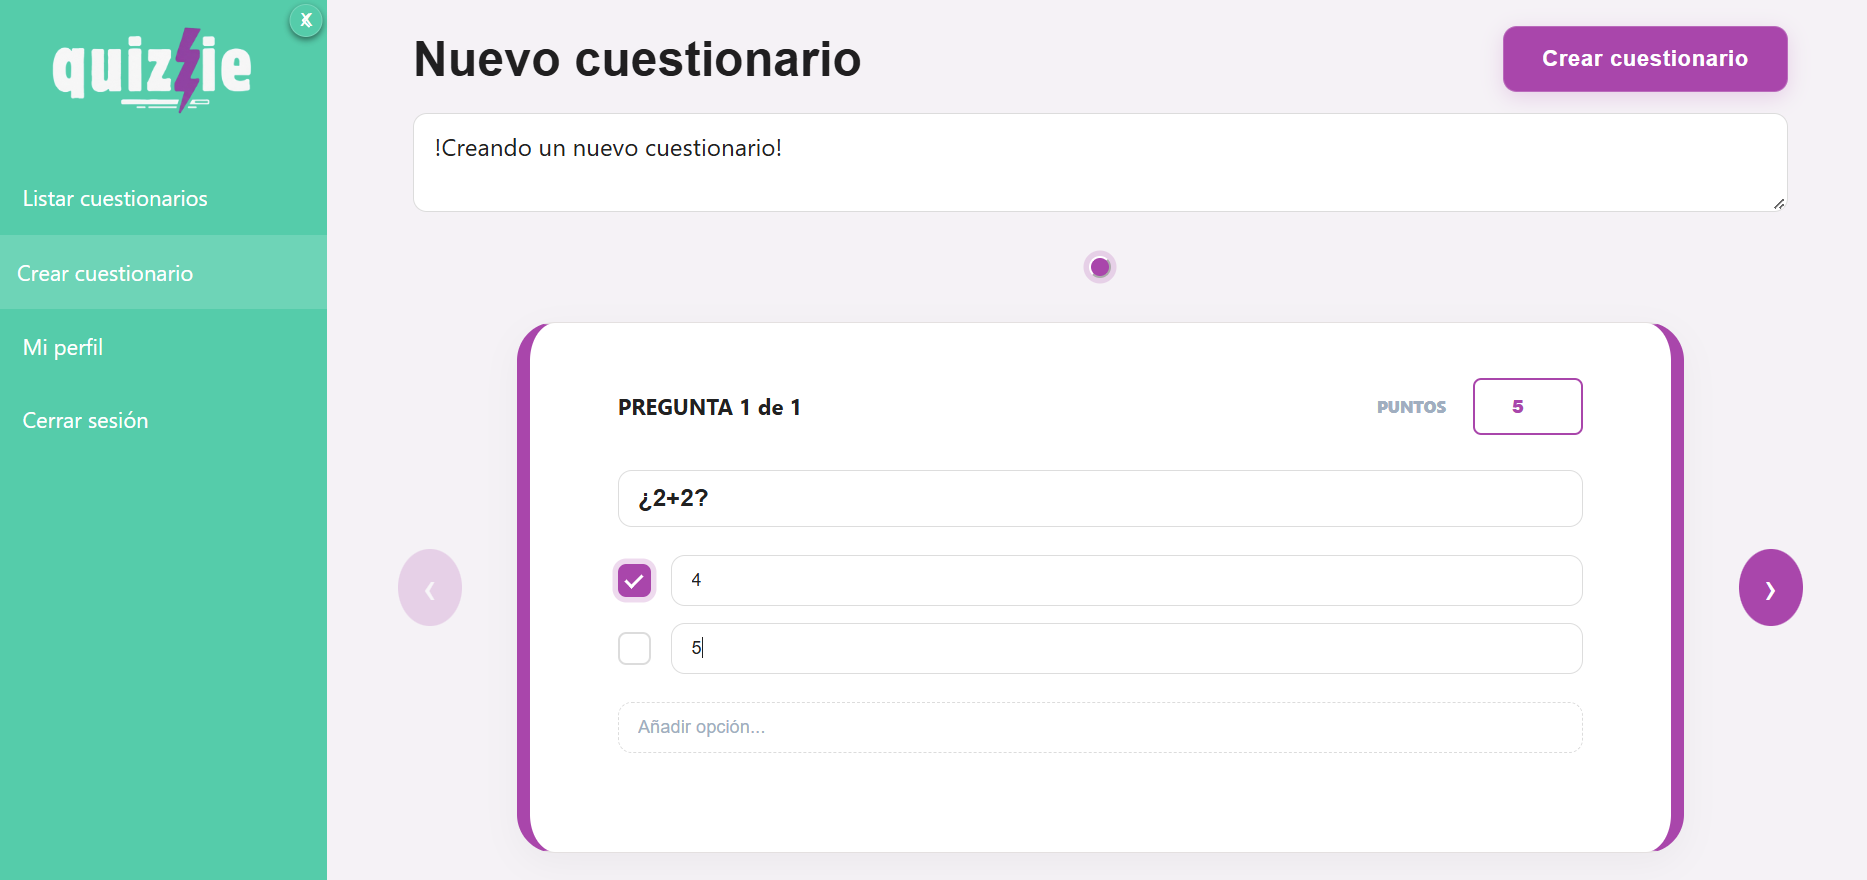
\includegraphics[width=1.1\textwidth]{screenshots/crear_cuestionario.png}%
  }
  \caption{Formulario para la creación de un nuevo cuestionario.}
  \label{fig:manual_crear_cuestionario}
\end{figure}

\subsection*{8. Visualización del catálogo filtrado}

Tras guardar los cambios, la nueva prueba queda registrada en el sistema y pasa a mostrarse dentro de la sección correspondiente en el catálogo de cuestionarios del usuario, lista para ser lanzada en una sala en directo.

\begin{figure}[H]
  \centering
  \makebox[\textwidth][c]{%
    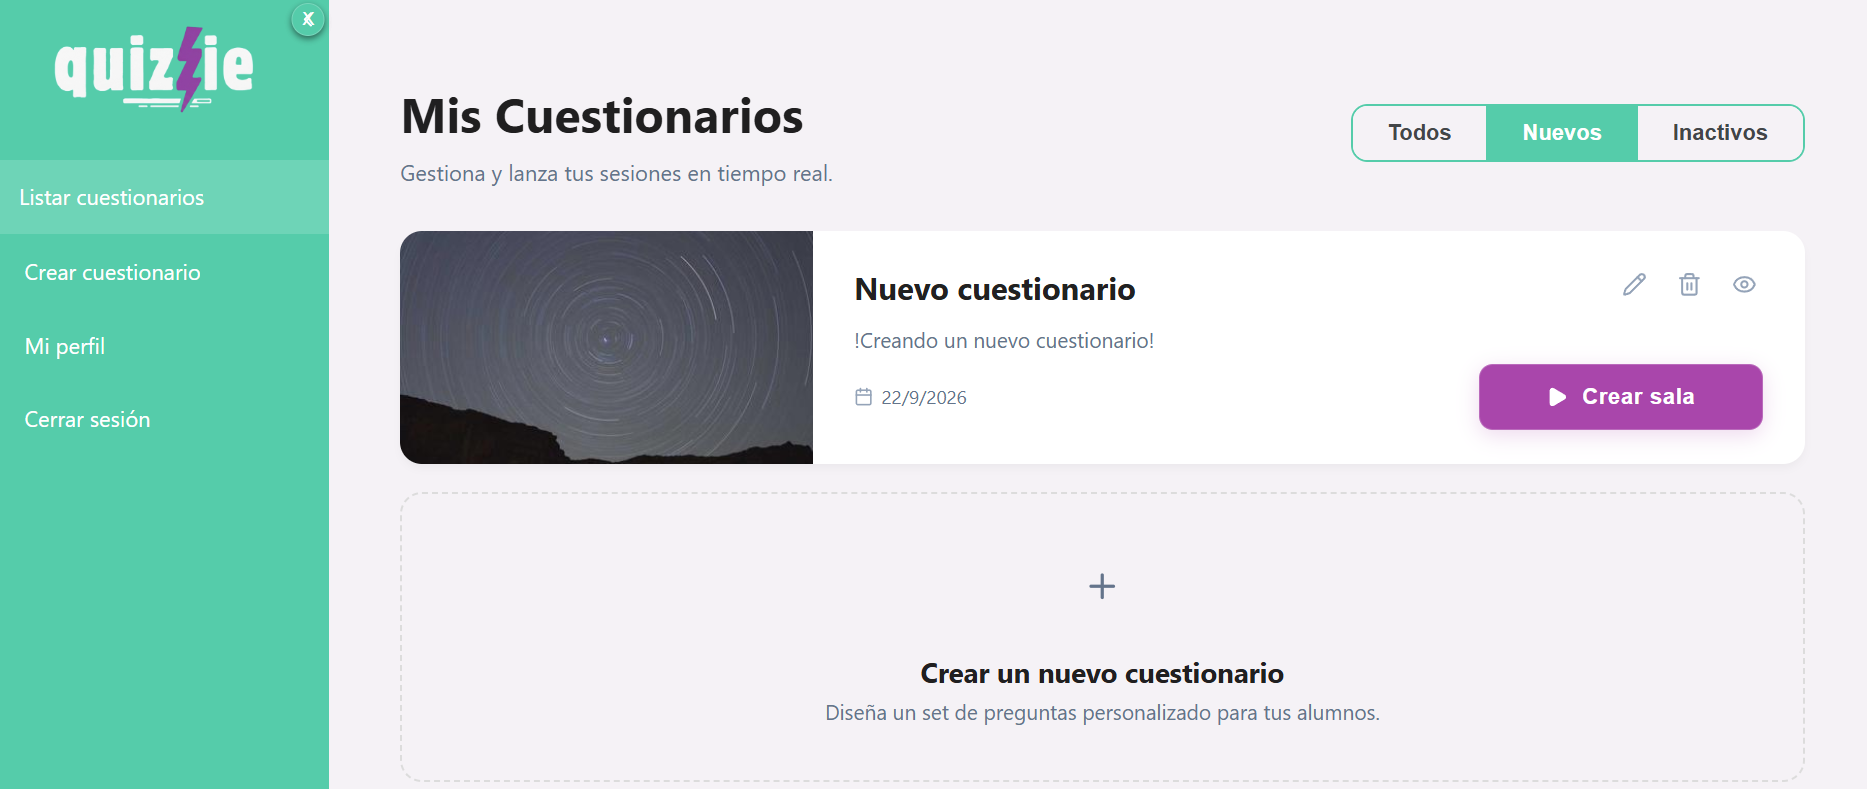
\includegraphics[width=1.1\textwidth]{screenshots/cuestionarios_nuevos.png}%
  }
  \caption{Cuestionario recién creado.}
  \label{fig:manual_cuestionarios_nuevos}
\end{figure}

\section*{Configuración, control de sala y verificación presencial}
\label{sec:manual_control_sala_en_directo}

Esta sección documenta el ciclo de vida completo de una sesión desde la perspectiva del profesor: desde el lanzamiento y parametrización de la sala, pasando por la orquestación de la partida en tiempo real, hasta la fase de verificación presencial mediante escaneo de códigos QR.

\subsection*{1. Selección de cuestionario y apertura de sala}

Desde la lista de cuestionarios, el profesor escoge la prueba que desea comenzar y pulsa sobre el botón para crear una nueva sala.

\begin{figure}[H]
  \centering
  \makebox[\textwidth][c]{%
    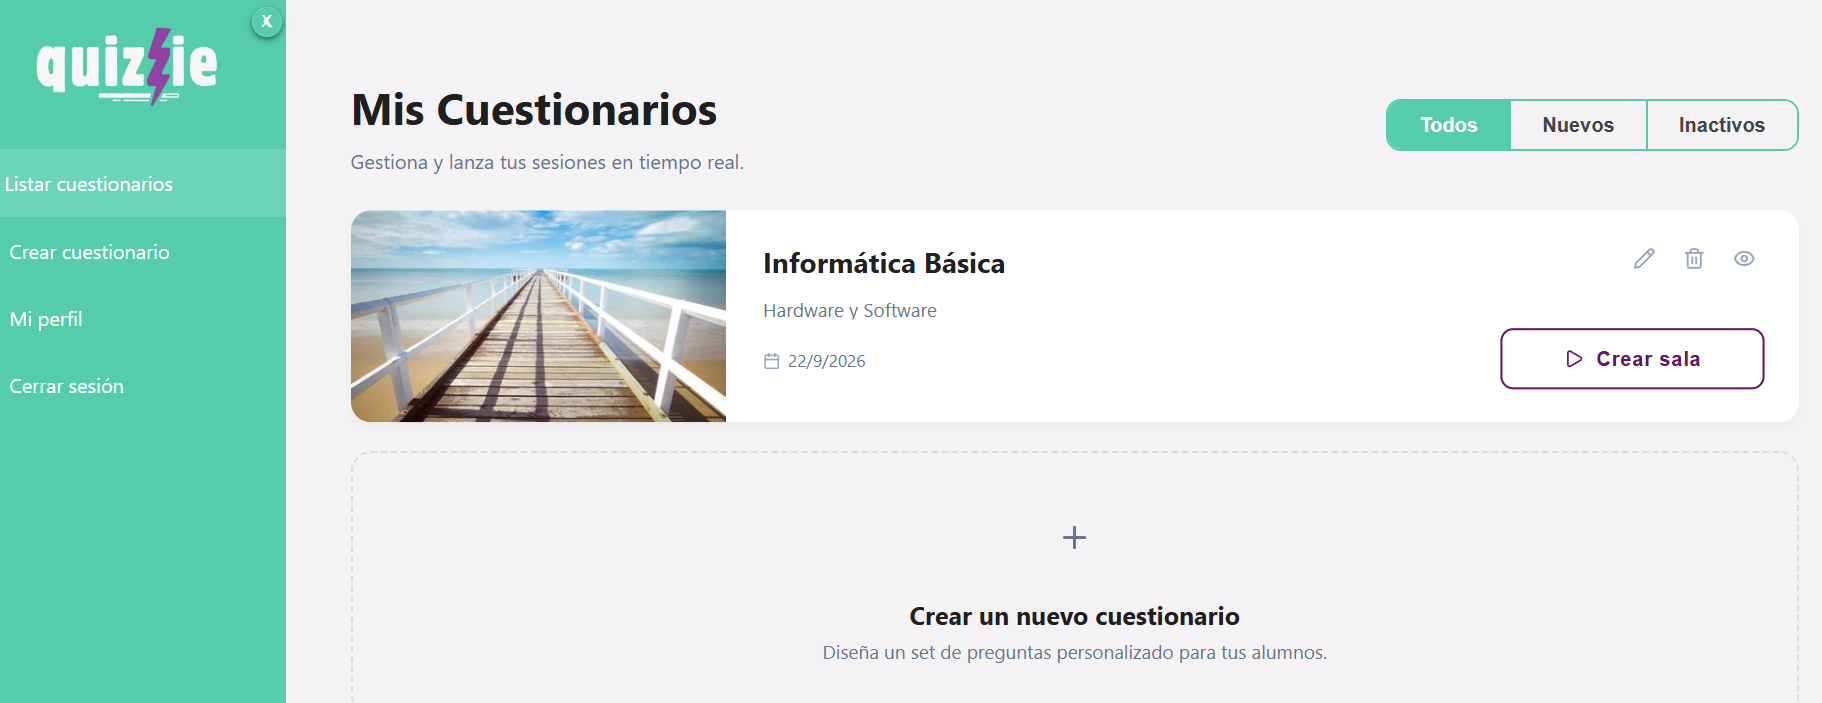
\includegraphics[width=1.1\textwidth]{screenshots/crear_sala.png}%
  }
  \caption{Selección de un cuestionario para inicializar una sala.}
  \label{fig:manual_crear_sala}
\end{figure}

\subsection*{2. Configuración de parámetros de la partida}

El profesor configura la dinámica de la partida a través de diversas opciones: orden aleatorio de preguntas, permutación aleatoria de opciones de respuesta para prevenir la copia entre estudiantes, visualización o no de rankings parciales tras cada pregunta (el ranking final siempre estará visible) y el tiempo límite concedido por pregunta. Al confirmar los parámetros, el sistema genera un código de acceso único y da paso a la sala de espera.

\begin{figure}[H]
  \centering
  \makebox[\textwidth][c]{%
    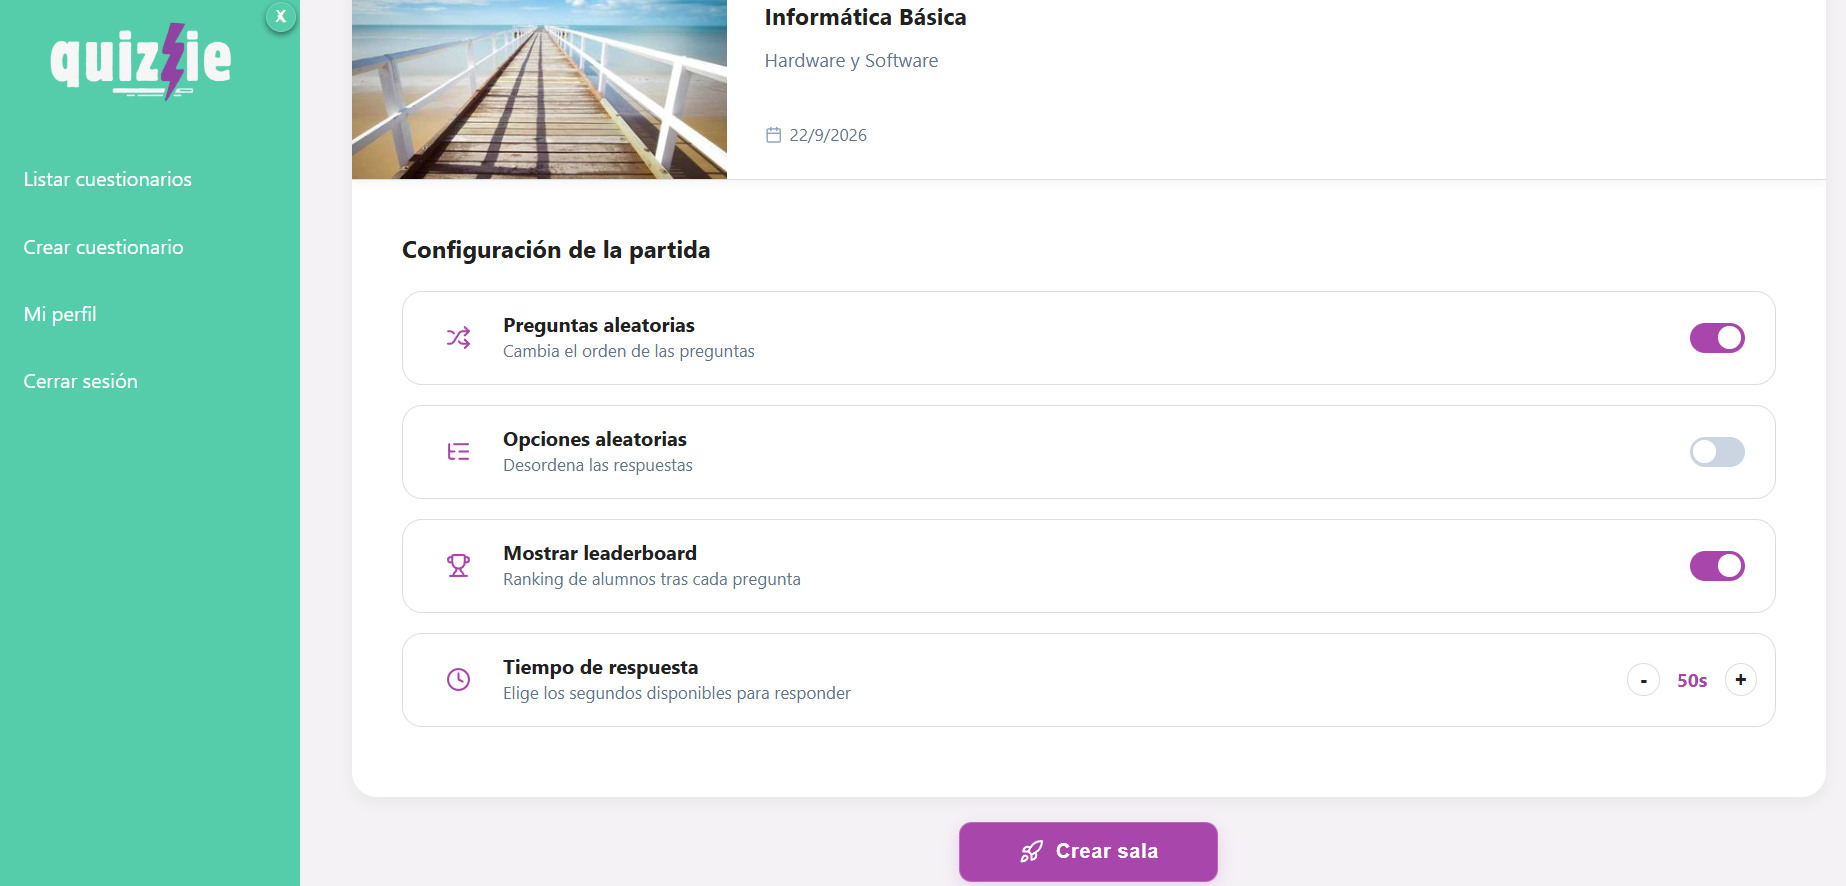
\includegraphics[width=1.1\textwidth]{screenshots/opciones_sala.png}%
  }
  \caption{Formulario de configuración de parámetros de la sala.}
  \label{fig:manual_opciones_sala}
\end{figure}

\subsection*{3. Sala de espera inicial}

La interfaz proyecta la sala de espera en su estado inicial vacío, exponiendo el código numérico PIN que el alumnado debe ingresar en sus dispositivos para vincularse a la sesión lectiva.

\begin{figure}[H]
  \centering
  \makebox[\textwidth][c]{%
    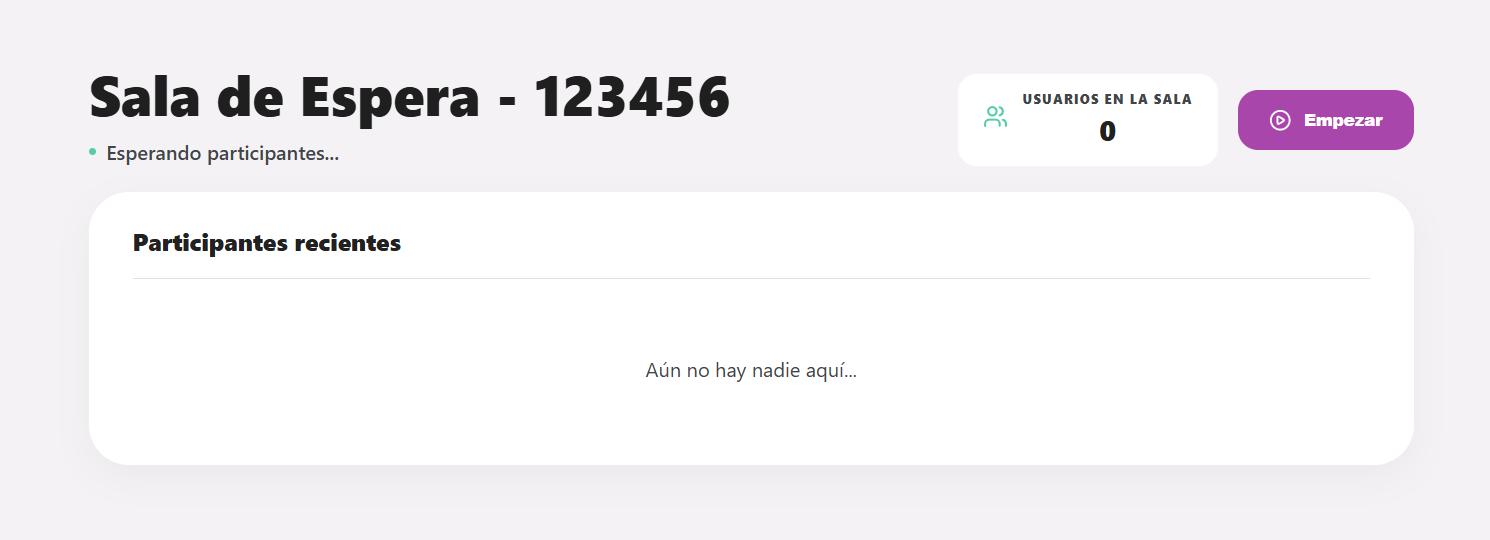
\includegraphics[width=1.1\textwidth]{screenshots/sala_espera_vacia.png}%
  }
  \caption{Sala de espera inicial a la espera de participantes.}
  \label{fig:manual_sala_espera_vacia}
\end{figure}

\subsection*{4. Incorporación de estudiantes y lanzamiento de la partida}

A medida que los estudiantes acceden a la sala, sus nombres o identificadores aparecen reflejados en pantalla. Cuando todos los asistentes se han incorporado, el profesor pulsa el botón para comenzar, dando paso a una breve cuenta atrás de sincronización previa al inicio de las preguntas.

\begin{figure}[H]
  \centering
  \makebox[\textwidth][c]{%
    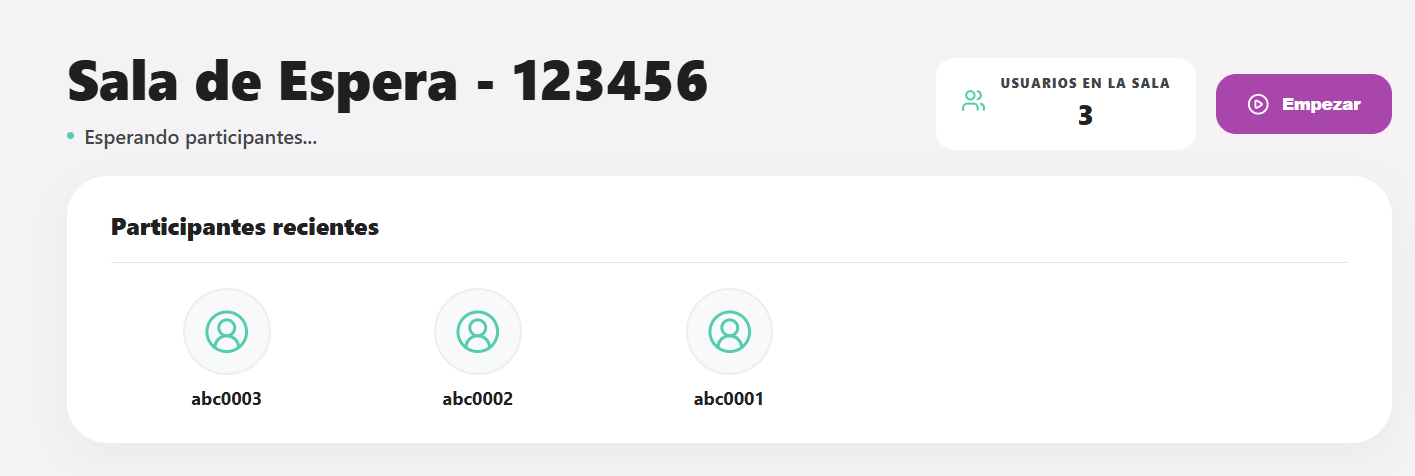
\includegraphics[width=1.1\textwidth]{screenshots/sala_espera.png}%
  }
  \caption{Sala de espera con estudiantes incorporados antes de iniciar.}
  \label{fig:manual_sala_espera}
\end{figure}

\subsection*{5. Fase de pregunta activa y recepción de respuestas}

Concluida la cuenta atrás, la plataforma proyecta el enunciado de la pregunta y el temporizador en cuenta regresiva según lo configurado. Los estudiantes solo pueden emitir respuestas mientras dicho reloj permanezca activo; si el temporizador se detiene o llega a cero, el sistema bloquea inmediatamente nuevos envíos.

\begin{figure}[H]
  \centering
  \makebox[\textwidth][c]{%
    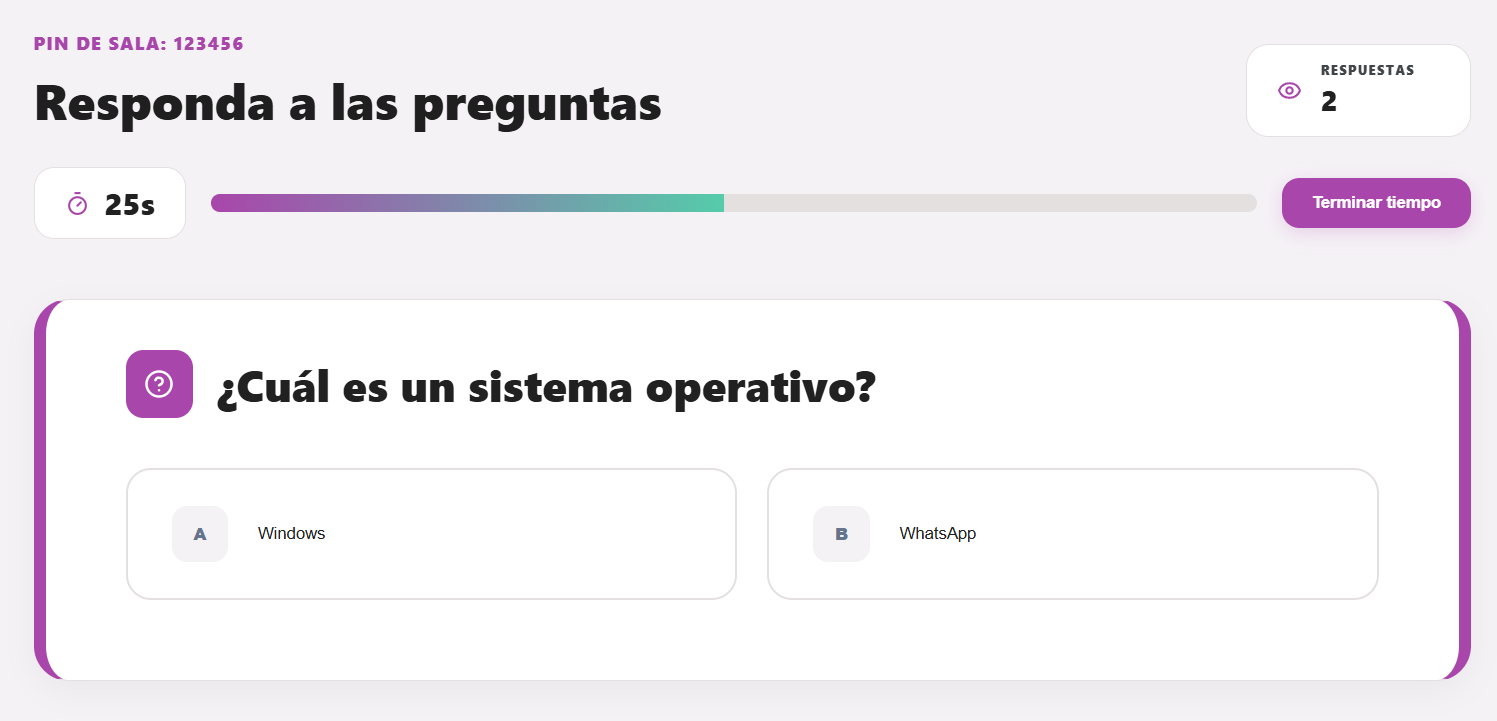
\includegraphics[width=1.1\textwidth]{screenshots/fase_respuesta_profesor.png}%
  }
  \caption{Pregunta proyectada en curso y temporizador activo.}
  \label{fig:manual_fase_respuesta_profesor}
\end{figure}

\subsection*{6. Tolerancia a fallos y reconexión del docente}

En caso de que el profesor sufra una pérdida de conexión de red o cierre accidentalmente la ventana, el sistema suspende de inmediato el temporizador para proteger la equidad de la prueba. Al volver a acceder a la plataforma, se ofrece la opción de reconexión directa a la sala activa, reanudándose el reloj y la interacción únicamente tras su regreso.

\begin{figure}[H]
  \centering
  \makebox[\textwidth][c]{%
    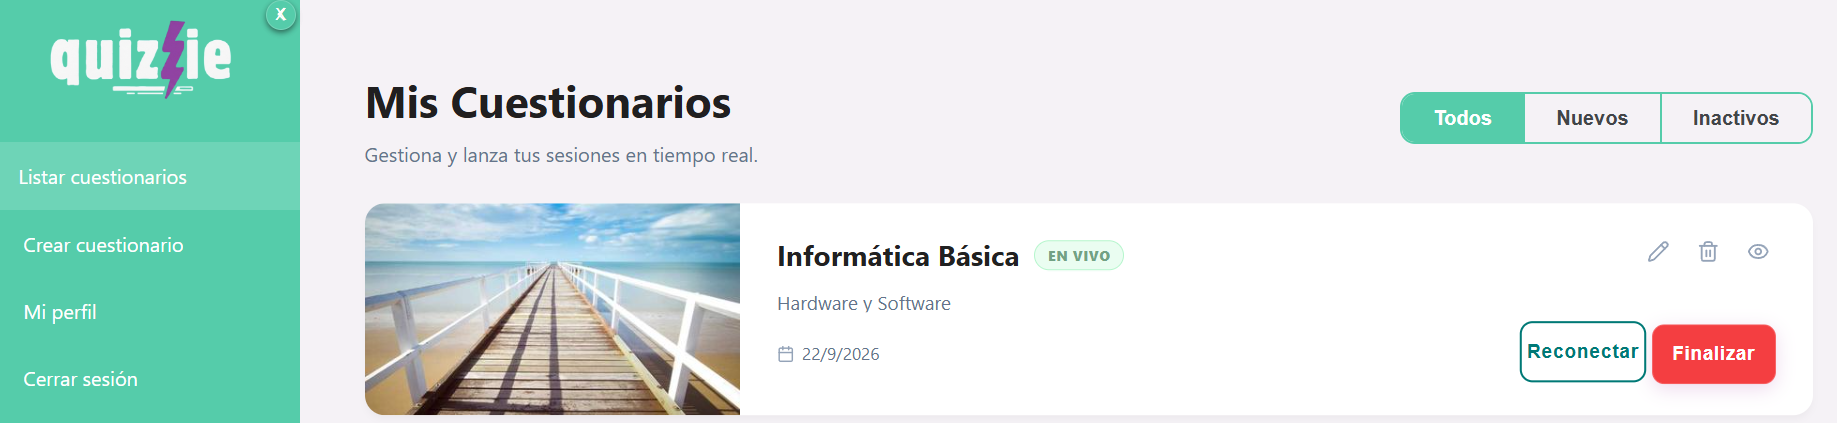
\includegraphics[width=1.1\textwidth]{screenshots/reconectarse_a_sala.png}%
  }
  \caption{Detección y recuperación de sesión activa tras desconexión.}
  \label{fig:manual_reconectarse_a_sala}
\end{figure}

\subsection*{7. Distribución analítica de respuestas}

Una vez agotado el tiempo de respuesta y al avanzar a la siguiente pantalla, el sistema proyecta una gráfica de barras con la distribución de las opciones elegidas por los alumnos. A partir de esta vista, y según las opciones configuradas inicialmente, se habilita la transición al ranking parcial o directamente a la siguiente pregunta o al final del cuestionario.

\begin{figure}[H]
  \centering
  \makebox[\textwidth][c]{%
    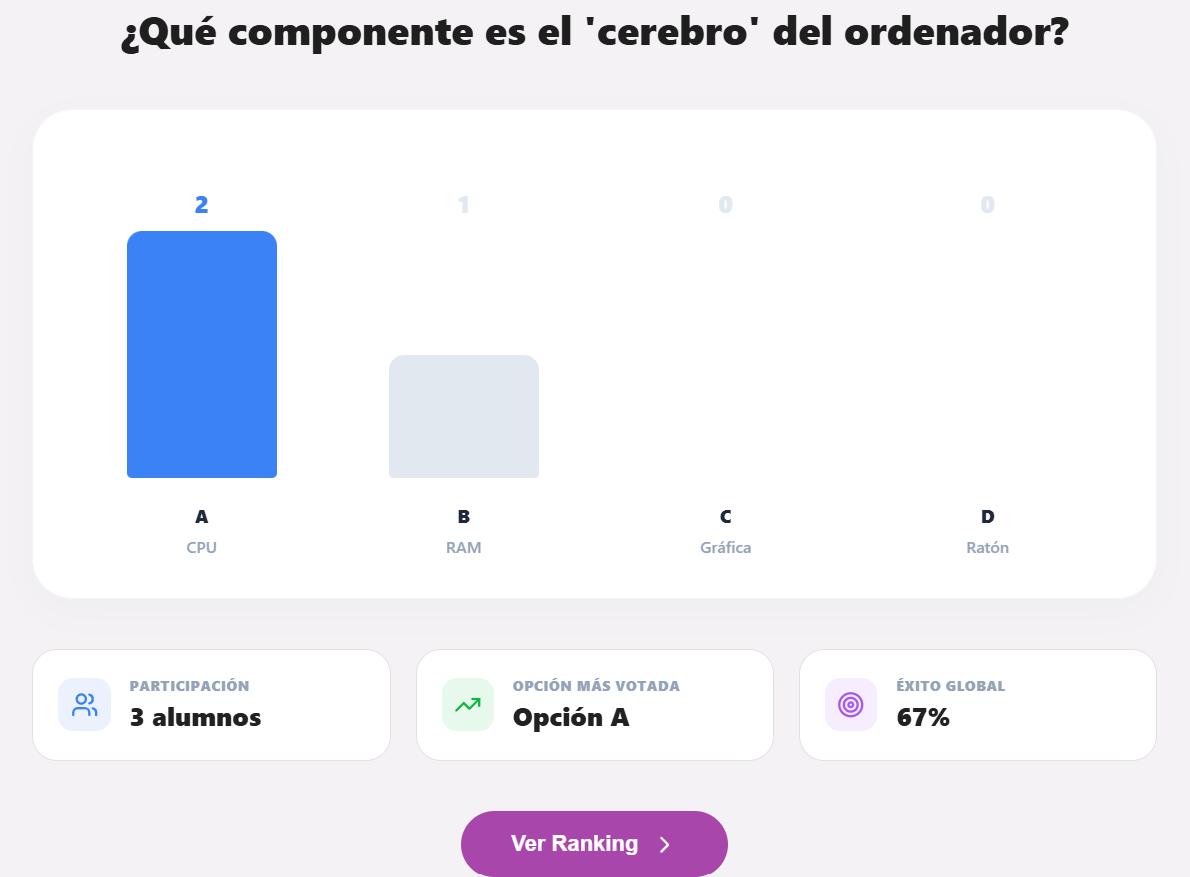
\includegraphics[width=0.9\textwidth]{screenshots/grafica_respuestas.png}%
  }
  \caption{Gráfica de distribución de respuestas seleccionadas por el alumnado.}
  \label{fig:manual_grafica_respuestas}
\end{figure}

\subsection*{8. Conclusión de la prueba y podio final}

Tras recorrer las rondas restantes de la evaluación, el sistema presenta la pantalla de podio final con las mejores calificaciones del aula. Al presionar el botón de finalización, la sala concluye su fase de preguntas y da paso al mecanismo de verificación presencial.

\begin{figure}[H]
  \centering
  \makebox[\textwidth][c]{%
    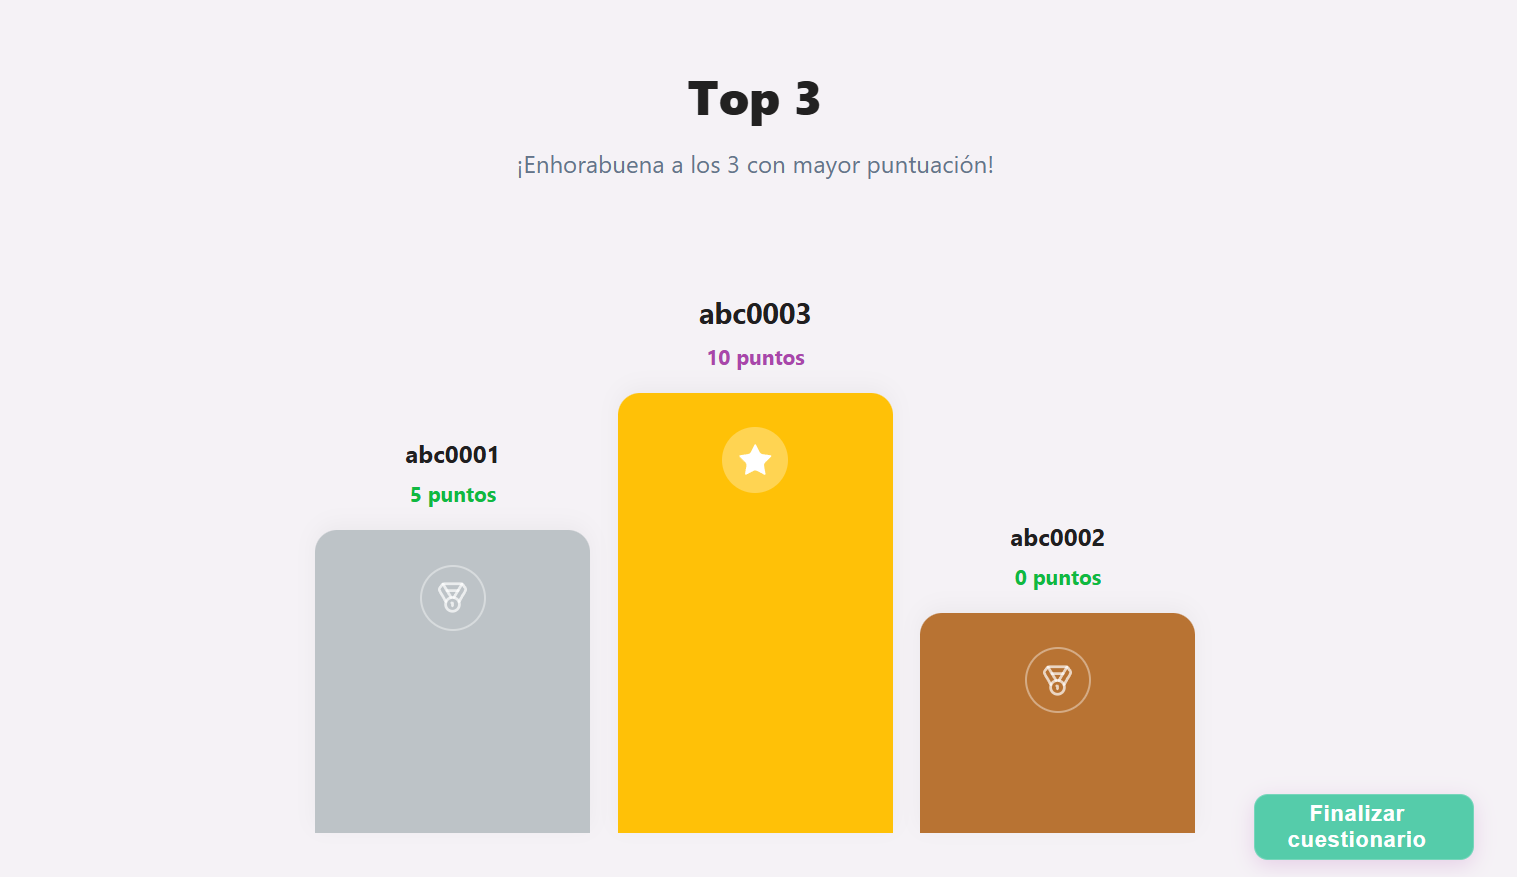
\includegraphics[width=0.9\textwidth]{screenshots/ranking_final.png}%
  }
  \caption{Podio de calificaciones globales al término de las preguntas.}
  \label{fig:manual_ranking_final}
\end{figure}

\subsection*{9. Panel de verificación presencial}

En esta fase, el profesor dispone de un panel con el listado de participantes para validar su asistencia física en el aula. Desde esta vista se habilita la acción para desplegar la interfaz de escaneo.

\begin{figure}[H]
  \centering
  \makebox[\textwidth][c]{%
    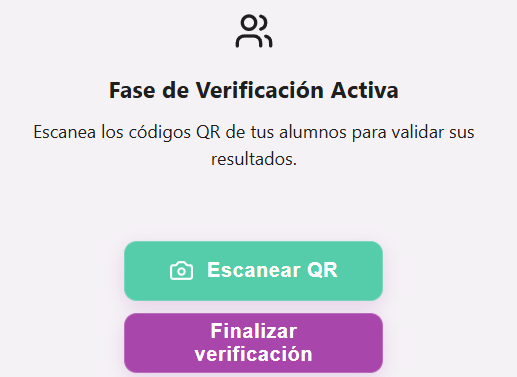
\includegraphics[width=0.55\textwidth]{screenshots/fase_verificacion.png}%
  }
  \caption{Panel para la verificación presencial de asistencia.}
  \label{fig:manual_fase_verificacion}
\end{figure}

\subsection*{10. Escáner y concesión de permisos de cámara}

Al solicitar la activación del lector de códigos, la aplicación despliega un diálogo modal que requiere la autorización del navegador para acceder a la cámara del dispositivo. Una vez concedido el permiso, el profesor procede al escaneo secuencial de los códigos QR mostrados en los dispositivos de los estudiantes para validar de forma fehaciente su presencialidad y asentar su nota.

\begin{figure}[H]
  \centering
  \makebox[\textwidth][c]{%
    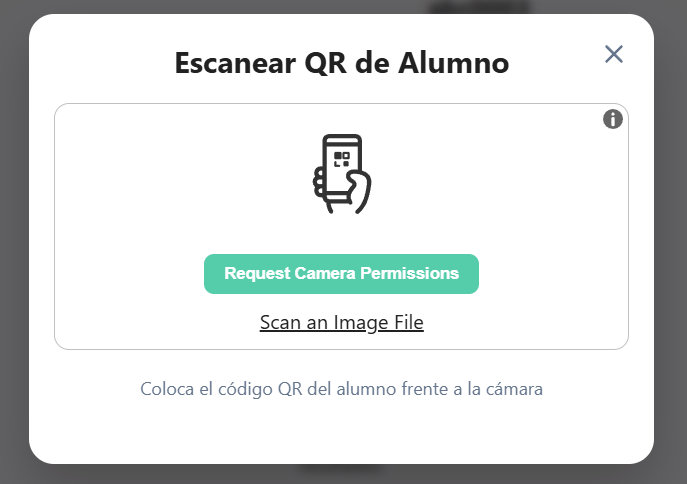
\includegraphics[width=0.6\textwidth]{screenshots/modal_verificacion.png}%
  }
  \caption{Diálogo modal de captura y solicitud de permisos de cámara.}
  \label{fig:manual_modal_verificacion}
\end{figure}

\end{appendices}